\documentclass[a4paper,12pt]{article}
\usepackage[top = 2.5cm, bottom = 2.5cm, left = 2.5cm, right = 2.5cm]{geometry}
\usepackage[T1]{fontenc}
\usepackage[utf8]{inputenc}
\usepackage{multirow} 
\usepackage{booktabs} 
\usepackage{graphicx}
\usepackage[spanish]{babel}
\usepackage{setspace}
\setlength{\parindent}{0in}
\usepackage{float}
\usepackage{fancyhdr}
\usepackage{amsmath}
\usepackage{amssymb}
\usepackage{amsthm}
\usepackage[numbers]{natbib}
\newcommand\Mycite[1]{%
	\citeauthor{#1}~[\citeyear{#1}]}
\usepackage{graphicx}
\usepackage{subcaption}
\usepackage{booktabs}
\usepackage{etoolbox}
\usepackage{minibox}
\usepackage{hyperref}
\usepackage{xcolor}
\usepackage[skins]{tcolorbox}
%---------------------------

\newtcolorbox{cajita}[1][]{
	 #1
}

\newenvironment{sol}
{\renewcommand\qedsymbol{$\square$}\begin{proof}[\textbf{Solución.}]}
	{\end{proof}}

\newenvironment{dem}
{\renewcommand\qedsymbol{$\blacksquare$}\begin{proof}[\textbf{Demostración.}]}
	{\end{proof}}

\newtheorem{problema}{Problema}
\newtheorem{definicion}{Definición}
\newtheorem{ejemplo}{Ejemplo}
\newtheorem{teorema}{Teorema}
\newtheorem{corolario}{Corolario}[teorema]
\newtheorem{lema}[teorema]{Lema}
\newtheorem{prop}{Proposición}
\newtheorem*{nota}{\textbf{NOTA}}
\renewcommand\qedsymbol{$\blacksquare$}
\usepackage{svg}
\usepackage{tikz}
\usepackage[framemethod=default]{mdframed}
\global\mdfdefinestyle{exampledefault}{%
linecolor=lightgray,linewidth=1pt,%
leftmargin=1cm,rightmargin=1cm,
}




\newenvironment{noter}[1]{%
\mdfsetup{%
frametitle={\tikz\node[fill=white,rectangle,inner sep=0pt,outer sep=0pt]{#1};},
frametitleaboveskip=-0.5\ht\strutbox,
frametitlealignment=\raggedright
}%
\begin{mdframed}[style=exampledefault]
}{\end{mdframed}}
\newcommand{\linea}{\noindent\rule{\textwidth}{3pt}}
\newcommand{\linita}{\noindent\rule{\textwidth}{1pt}}

\AtBeginEnvironment{align}{\setcounter{equation}{0}}
\pagestyle{fancy}

\fancyhf{}









%----------------------------------------------------------
\lhead{\footnotesize Modelación y Simulación}
\rhead{\footnotesize  Rudik Roberto Rompich}
\cfoot{\footnotesize \thepage}


%--------------------------

\begin{document}
 \thispagestyle{empty} 
    \begin{tabular}{p{15.5cm}}
    \begin{tabbing}
    \textbf{Universidad del Valle de Guatemala} \\
    Departamento de Matemática\\
    Licenciatura en Matemática Aplicada\\\\
   \textbf{Estudiante:} Rudik Roberto Rompich\\
   \textbf{Correo:}  \href{mailto:rom19857@uvg.edu.gt}{rom19857@uvg.edu.gt}\\
   \textbf{Carné:} 19857
    \end{tabbing}
    \begin{center}
        CC3039 - Modelación y Simulación - Catedrático: Oseas Paredes\\
        \today
    \end{center}\\
    \hline
    \\
    \end{tabular} 
    \vspace*{0.3cm} 
    \begin{center} 
    {\Large \bf Microproyecto 1
} 
        \vspace{2mm}
    \end{center}
    \vspace{0.4cm}
%--------------------------

\begin{problema}
	Willow Brook National opera un cajero automático en el que los clientes realizan transacciones bancarias sin descender de sus automóviles. En las mañanas de días hábiles, las llegadas al auto cajero ocurren al azar, con una tasa de llegadas de 24 clientes por hora o 0.4 clientes por minuto.
	\begin{enumerate}
		\item ¿Cuál es la medida o el número esperado de clientes que llegará en un lapso de cinco minutos?
		\begin{sol}
			Como estamos basando $\lambda=$ 0.4 clientes por minuto, entonces los clientes esperados que podrían llegar en 5 minutos son: 
			
			$$0.4*5= 2 \text{ personas.}$$
			
		
		\end{sol}
		\item Suponga que puede usarse la distribución de probabilidad de Poisson para describir el proceso de llegadas. Utilice la tasa de llegadas de la parte a) para calcular las probabilidades de que exactamente 0, 1, 2 y 3 clientes lleguen durante un lapso de cinco minutos.
		\begin{sol}
			Dado la función de probabilidad de Poisson, 
			$$P(x)=\frac{\lambda^x e^{-\lambda}}{x!}\implies P(x)=\frac{(2)^x e^{-2}}{x!}, \quad x=0,1,2,\cdots$$
			Tenemos, 
			\begin{align*}
				P(0) &= \frac{(2)^0 e^{-2}}{0!}=0.1353 \\
				P(1) &= \frac{(2)^1 e^{-2}}{1!}= 0.2707\\
				P(2) &= \frac{(2)^2 e^{-2}}{2!}=0.2707\\
				P(3) &= \frac{(2)^3 e^{-2}}{3!}= 0.1804\\
			\end{align*}
		\end{sol}
		\item ¿Se esperan demoras si más de tres clientes llegan durante cualquier lapso de cinco minutos? ¿Cuál es la probabilidad de que ocurran demoras?
		\begin{sol}
			La probabilidad de demoras se puede calcular como: 
			$$P(x>3)= 1- P(x\leq 3)= 1- [P(0)+P(1)+P(2)+P(3)]= 1- 0.8571= 0.1429$$
			Por lo tanto, la probabilidad de demora cuando hay más de 3 clientes es de 14.29\%.  
		\end{sol}
	\end{enumerate}	
\end{problema}


\begin{problema}
	En el sistema de línea de espera del Willow Brook National Bank (vea el problema 1), suponga que los tiempos de servicio del auto cajero siguen una distribución de probabilidad exponencial con una tasa de servicios de 36 clientes por hora, o 0.6 clientes por minuto.
\begin{cajita}
	Distribución de probabilidad exponencial dada por, 
	$$P(\text{tiempo de servicio}\leq t)=1- e^{-\mu t}=1- e^{-0.6 t}$$
\end{cajita}
	 Utilice la distribución de probabilidad exponencial para responder las siguientes preguntas:
	 
	\begin{enumerate}
		\item ¿Cuál es la probabilidad de que el tiempo de servicio sea de un minuto o menos?
		\begin{sol}
			$$P(\text{tiempo de servicio}\leq 1)=1- e^{-0.6* 1}= 0.4512$$
		\end{sol}
		\item ¿Cuál es la probabilidad de que el tiempo de servicio sea de dos minutos o menos?
		\begin{sol}
			$$P(\text{tiempo de servicio}\leq 2)=1- e^{-0.6*  2}=0.6988$$
		\end{sol}
		\item ¿Cuál es la probabilidad de que el tiempo de servicio sea de más de dos minutos?
		\begin{sol}
			$$P(\text{tiempo de servicio}>2)=e^{-0.6* 2}=0.3012$$
		\end{sol}
	\end{enumerate}
\end{problema}


\begin{problema}
	Utilice la operación del auto cajero de canal único referida en los problemas 1 y 2 para determinar las siguientes características de operación del sistema:
	\begin{figure}[H]
		\centering
		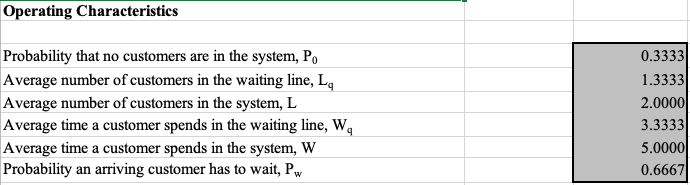
\includegraphics[scale=0.5]{Images/3}
		\caption{Plantilla de Quantitative Methods for Business de Andersen et al. }
	\end{figure}
	\begin{enumerate}
		\item La probabilidad de que no haya clientes en el sistema.
		\begin{sol}
			$$P_0=1-\lambda/\mu = 1-0.4/0.6=0.33$$
		\end{sol}
		\item El número promedio de clientes que esperan.
			\begin{sol}
			$$L_q=\lambda^2 / [\mu(\mu -\lambda)]=0.16/0.12=1.333$$
				\end{sol}
		\item El número promedio de clientes en el sistema.
			\begin{sol}
			$$L=L_q+\lambda/\mu=1.333+0.4/0.6=2$$
		\end{sol}
		\item El tiempo promedio que un cliente pasa esperando.
			\begin{sol}
			$$W_q=L_q/\lambda=1.333/0.4= 3.33 \text{ minutos}$$
		\end{sol}
		\item El tiempo promedio que un cliente pasa en el sistema.
			\begin{sol}
			$$W=W_q+1/\mu =3.333+1/0.6=5 \text{ minutos}$$
		\end{sol}
		\item La probabilidad de que los clientes que llegan tengan que esperar a que los atiendan.
			\begin{sol}
			$$P_W=\lambda/\mu = 0.4/0.6= 0.6667$$
		\end{sol}
	\end{enumerate}

\end{problema}

	


\begin{problema}
	Utilice la operación del auto cajero de canal único referida en los problemas 1-3 para determinar las probabilidades de que 0, 1, 2 y 3 clientes estén en el sistema. ¿Cuál es la probabilidad de que más de tres clientes estén en el auto cajero al mismo tiempo?
\end{problema}
\begin{sol}
	La probabilidad de $n$ unidades se calcula con: 
	$$P_n=\left(\frac{\lambda}{\mu}\right)^n *P_0=\left(\frac{0.4}{0.6}\right)^n *0.333$$
	Entonces, las probabilidad para 0,1,2 y 3: 
	\begin{align*}
		P_0&=\left(\frac{0.4}{0.6}\right)^0 *0.3333 = 0.3333\\
		P_1&=\left(\frac{0.4}{0.6}\right)^1*0.3333=0.2222\\
		P_2&=\left(\frac{0.4}{0.6}\right)^2 *0.3333=0.1481\\
		P_3&=\left(\frac{0.4}{0.6}\right)^3 *0.3333=0.0988
	\end{align*}
Ahora, la probabilidad mayor a 3 clientes: 
$$P(n>3)=1-P(n\leq 3)=1-[P_0+P_1+P_2+P_3]=1- 0.8024=0.1976 $$
\end{sol}


\begin{problema}
	El escritorio de referencia de la biblioteca de una universidad recibe peticiones de ayuda. Suponga que puede utilizarse una distribución de probabilidad de Poisson con una tasa de llegadas de 10 peticiones por hora para describir el patrón de llegadas y de que los tiempos de servicio sigan una distribución de probabilidad exponencial con una tasa de servicios de 12 peticiones por hora.
	\begin{figure}[H]
		\centering
		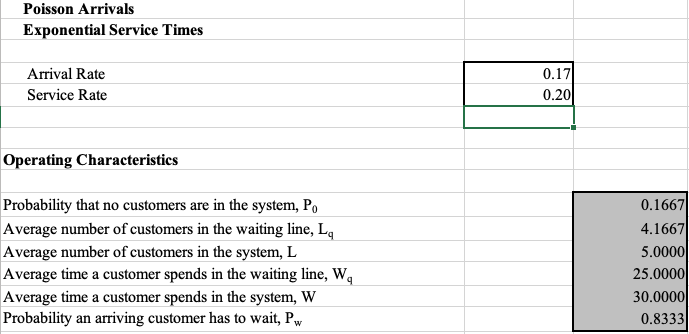
\includegraphics[scale=0.5]{Images/5}
		\caption{Plantilla de Quantitative Methods for Business de Andersen et al. }
	\end{figure}
	\begin{enumerate}
		\item ¿Cuál es la probabilidad de que no haya peticiones de ayuda en el sistema?
		\begin{dem}
			$$P_0=0.1667$$
		\end{dem}
		\item ¿Cuál es el número promedio de peticiones que esperan ser atendidas?
		\begin{dem}
			$$L_q= 4.1667$$
		\end{dem}
		\item ¿Cuál es el tiempo de espera promedio en minutos antes de que comience a ser atendido?
		\begin{dem}
			$$W_q = 25 \text{ minutos}$$
		\end{dem}
		\item ¿Cuál es el tiempo promedio en el escritorio de referencia en minutos (tiempo de espera más tiempo de servicio)?
		\begin{dem}
			$$W= 30 \text{ minutos}$$
		\end{dem}
		\item ¿Cuál es la probabilidad de que una nueva llegada tenga que esperar a que la atiendan?
		\begin{dem}
			$$P_w = 0.8333$$
		\end{dem}
	\end{enumerate}
\end{problema}

%---------------------------
%\bibliographystyle{apa}
%\bibliography{referencias.bib}

\end{document}